\input{Packages}
\input{Definitions}
\DeclareRobustCommand{\stirling}{\genfrac\{\}{0pt}{}}
%this removes numbering from the section, from some reason the \section*{} command doesnt work once you redefine it
\setcounter{secnumdepth}{0} 

% Define variables for week number and meeting date
\newcommand{\weekNum}{8} % Change this to update the week number
\newcommand{\meetingDate}{Mar 12, 2025} 

\begin{document}
\pagestyle{empty}
\sloppy
\maketitle

\section{Topic: Invariants \& Constructions}

% https://www.math.cmu.edu/~mlavrov/arml/15-16/proofs-02-28-16.pdf
\begin{problem}[C][2][Western PA ARML Practice/2]
    %Discrete ^ Invariants
    The numbers $1, 2, \ldots , 100$ are written on a blackboard. You may choose any two numbers $a$ and $b$ and erase them, replacing them with the single number $a + b - 1$. After 99 steps, only a single number will be left. What is it?
\end{problem}

\begin{problem}[C][3][Engel]
    %Construction ^ Discrete 
    There is a positive integer in each square of a rectangular table. In each move, you may double each number in a row or subtract 1 from each number of a column. Prove that you can reach a table of zeroes by a sequence of these permitted moves.
\end{problem}

\begin{problem}[C][3][A Dramatic Nim Game]
    %Construction ^ Nim games
    Deep within the Academy of Raya Lucaria, aspiring sorcerers must prove their intellect in a legendary test known as the Trial of Glintstone Embers. In the Grand Library, two scholars \emph{take turns} siphoning 1, 2, or 3 embers from an enchanted brazier containing 2025 embers. The scholar who takes the last ember will see beyond the secrets of Rennala’s full moon, gaining the favor of the academy’s greatest minds. Tonight, you stand before the brazier, facing a rival scholar. So sure of himself, he gives you the first turn. Can you devise a winning strategy, or will you be left in the dark?
\end{problem}

\begin{problem}[C][5][Swiss Olympiad 2010]
    %Discrete ^ Invariants
    Three coins lie on integer points on the number line. A move consists of choosing and moving two coins, the first one 1 unit to the right and the second one 1 unit to the left. Under which initial conditions is it possible to move all coins to one single point?
\end{problem}

\begin{problem}[C][1][The so-called Pigeon-Hole Principle]
    %Discrete ^ Pigeon-Hole Principle
    Show that among any eight positive integers, we can always find two whose sum or difference is a multiple of twelve. Is the same argument true if we select seven positive integers instead?
\end{problem}

\begin{solution}
    just leaving this here so we remember to turn solutions off when printing
\end{solution}

\begin{problem}[C][3][BMT 2021 Discrete/3]
    %Discrete ^ Counting
    How many distinct sums can be made from adding together exactly 8 numbers that are chosen from the set $\{1,4,7,10\}$, where each number in the set is chosen at least once? (For example, one possible sum is $1 + 1 + 1 + 4 + 7 + 7 + 10 + 10 = 41$.)
\end{problem}

\begin{problem}[C][4][NIMO Winter 2014/3]
    %Discrete ^ Invariants
     The numbers $1$, $2$, \dots, $10$ are written on a board.
  Every minute, one can select three numbers
  $a$, $b$, $c$ on the board, erase them,
  and write $\sqrt{a^2+b^2+c^2}$ in their place.
  This process continues until no more numbers can be erased.
  What is the largest possible number
  that can remain on the board at this point?
\end{problem}

%\begin{problem}[C][3][A Walk Through Combinatorics]
    %%Discrete ^ Pigeon-Hole Principle
    %The set $M$ consists of nine positive integers, none of which has a prime divisor larger than six. %Prove that $M$ has two elements whose product is the square of an integer.
%\end{problem}

%\begin{problem}[C][2][BAMO 2024/1]
    %Discrete ^ Algebra 
    %Sugar Station sells 44 different kinds of candies, packaged one to a box. Each box is priced at a positive integer number of cents, and it costs \$1.51 to buy one of every kind. (There is no discount based on the number of candies in a purchase.) Unfortunately, Anna only has \$0.75.
    
    %\begin{itemize}
        %\item[a)] Show that Anna can buy at least 22 boxes, each containing a different candy.
        %\item[b)] Show that Anna can do even better, buying at least 25 boxes, each containing a different candy
    %\end{itemize}
%\end{problem}

%\begin{problem}[C][2]
    %%Discrete ^ Pigeon-Hole Principle
    %Show that if we select 5 points inside a square of length $1$, there is at least two points whose %distance is at most $\sqrt{2}/2$.
%\end{problem}

\begin{problem}[C][4][Cuba 2022/6]
    %Discrete ^ Invariants
    On the board are written the positive integers $1, 2, \ldots, 2022$. Alex and Sophia have the chance of making the next movement:
    They can select two of the numbers on the board, say $\alpha, \beta$ and substitute them for the numbers $4 \alpha - \beta, 7 \beta - 8 \alpha$. Alex claims that after a finite number of moves, it is possible that the numbers on the board are $3, 6, 9, \ldots 6066$. Sophia claims that this is impossible. Who is right?
\end{problem}

\begin{problem}[C][6][BAMO 2024/2]
    %Discrete ^ Construction
    Sasha wants to bake 6 cookies in his 8 inch × 8 inch square baking sheet. With a cookie cutter, he cuts out from the dough six circular shapes, each exactly 3 inches in diameter. Can he place these six dough shapes on the baking sheet without the shapes touching each other? If yes, show us how. If no, explain why not. (Assume that the dough does not expand during baking.)
\end{problem}


\begin{problem}[C][3][MP4G 2024/14]
    %Discrete ^ Counting ^ MinMax ^ Construction
    The set $S$ contains $2024$ elements. What is the size of a largest collection $C$ of subsets of $S$ with the property that the intersection of every three subsets in $C$ is nonempty,
  but the intersection of every four is empty?
\end{problem}


%\newpage %I did a page-break here to not separate problem 8. 
\begin{problem}[C][8][OTIS Mock AIME I 2025/9]
    %Discrete ^ Counting
    Winston forgot the definition of a prime number. He instead defines a New-prime recursively as follows:
\begin{itemize}
    \item \(1\) is not New-prime.
    \item A positive integer \( n > 1 \) is New-prime if and only if \( n \) cannot be expressed as the product of exactly two (not necessarily distinct) New-prime positive integers.
\end{itemize}
Compute the number of positive integers dividing \(50054\) which are New-primes.

\end{problem}

%\begin{problem}[C][5][BAMO 2013/4]
    %For a positive integer $n \geq 2$, consider the $n-1$ fractions
    %$$ \frac{2}{1}, \frac{3}{2}, \ldots, \frac{n}{n-1}$$
    %The product of these fractions equals $n$, but if you reciprocate (i.e. turn upside down) some of the fractions, the product will change. Can you make the product equal 1? Find all values of $n$ for which this is possible and prove that you have found them all
%\end{problem}

\section{Other Fun Stuff}\setcounter{problem}{0}

% \begin{problem}[Z][3][BMT 2023 Discrete/3]
%     Find the number of positive integers $n$ less than 10000 such that there are more 4’s in the digits of $n+1$ than in the digits of $n$.
% \end{problem}

\begin{problem}[Z][3][BmMT 2015 Individual/7]
    %Divisibility ^ Digits
    A three digit number is a multiple of 35 and the sum of its digits is 15. Find this number.
\end{problem}

\begin{problem}[Z][5][AMATYC Fall 2013/4]
    %Discrete
    The digits of a number are rearranged, and the resulting number is added to the original number. Consider the following values:\smallbreak
    \hspace{25pt}777\hfill7,777\hfill77,777\hfill777,777\hfill7,777,777\hspace{25pt}\smallbreak

    How many of the numbers above could NOT equal this sum?
    \end{problem}
    \multOpt[5]{0}[1][2][3][4]

\begin{problem}[Z][5][AMATYC Fall 2013/10]
    %Knights and Knaves ^ Discrete
    Knaves always lie; knights always tell the truth. Al says, “Bo is a knight,” Bo says, “Cy is a knave,” and Cy says, “Exactly one of Al and Bo is a knave." If Al, Bo, and Cy are each either a knight or a knave, it is true that
\end{problem}\smallbreak\vspace{2pt}
\begin{tabular}{r@{ }l @{\hskip 1cm} r@{ }l}
    A. & Al and Cy are both knights  & B. & Al and Cy are both knaves \\
    C. & Al is a knight, Cy is a knave  & D. & Al is a knave, Cy is a knight \\
    E. & it cannot be determined what Al and Cy are &
\end{tabular}

\begin{problem}[Z][2][BMT 2020 Calculus/6]
    %Calculus ^ Derivatives
    For some $a > 1$, the curves $y = a^x$ and $y = \log_a(x)$ are tangent to each other at exactly one point. Compute $| \ln(\ln(a))|$.
\end{problem}

\begin{problem}[Z][4][BmMT 2015 Individual/18]\par\vspace{-7pt}
    %Geometry
    \begin{minipage}[t]{0.7\linewidth}\vspace{0pt}
    Assume that $A,B,C,D,E,F$ are equally spaced on a circle of radius 1, as in the figure on the right. Find the area of the kite bounded by the lines $EA, AC, F C, BE$.
    \end{minipage}\hfill
    \begin{minipage}[t]{0.3\linewidth}\vspace{-30pt}
    \hfill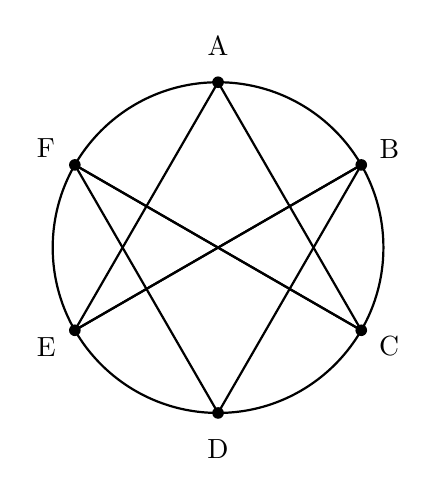
\begin{tikzpicture}[scale=0.7]
        % Define circle radius
        \def\r{3}
    
        % Define points on the circle
        \foreach \i/\name in {90/A, 30/B, -30/C, -90/D, -150/E, 150/F}
        {
            \coordinate (\name) at (\i:\r);
            \fill (\name) circle(3pt);
            \node[anchor=\i] at (\i:{\r+1}) {\name};
        }
            %\fill (\name) circle(2pt) node[above right] {\name};
    
        % Draw the circle
        \draw[thick] (0,0) circle(\r);
    
        % Draw the points
        % \foreach \name in {A, B, C, D, E, F}
        %     \fill (\name) circle(2pt) node[above right] {\name};
    
        % Draw connecting lines
        \draw[thick] (E) -- (A);
        \draw[thick] (A) -- (C);
        \draw[thick] (F) -- (C);
        \draw[thick] (B) -- (E);
        
        % Additional lines for the pattern
        \draw[thick] (B) -- (E);
        \draw[thick] (C) -- (F);
        \draw[thick] (D) -- (F);
        \draw[thick] (B) -- (D);            
    \end{tikzpicture}\hfill
\end{minipage}
\end{problem}

%Saying Discrete is too wide, i was planning on also doing Discrete next week, i might remove some of the problems i added -- edgar

\end{document}